\section{Control}
\label{sec:control}

% The control will be done with vector control also known as field orientated control (FOC) where the motor currents are transformed from three-phase AC signals to a single vector in a rotating dp-frame with a Clarke and a Park transformation. The controller is placed in the dq-frame and its output signals are converted from a rotating vector in the dq-frame back to a signal for each inverter phase.
The section will go through which control type has been chosen, how it works and how it is used. Then the motor model is setup and explained and lastly the motor controller is designed.

\subsection{Simplified motor model}
The motor is a \textit{Motenergy ME1117 PMAC Motor}. Its parameters can be seen in table \ref{Motor_parameters_list}.

\begin{table} [H]
    \centering
    \begin{tabular}{|c|c|} \cline{1-2}
        \textbf{Parameters} & \textbf{Number} \\ \cline{1-2}
        \textbf{Pole pair} & $4\ pairs\ (8\ poles)$ \\ \cline{1-2}
        \textbf{Phase to Phase R} & $0.013\ohm$ \\ \cline{1-2}
        \textbf{Maximum rotational speed} & $5000$ \textit{RPM} \\ \cline{1-2}
        \textbf{Voltage rating} & $0-76$ \textit{Volts} \\ \cline{1-2}
        \textbf{Torque constant} & $0.13$ \textit{Nm/A} \\ \cline{1-2}
        \textbf{Inductance Phase to Phase} & $0.1$ \textit{mH} \\ \cline{1-2}
        \textbf{Armature Inertia} & $52\ kg/cm^2$ \\ \cline{1-2}
        \textbf{Continuous current} & $100\ A$ \\ \cline{1-2}
        \textbf{Peak Current for 1 min} & $300\ A$ \\ \cline{1-2}  
    \end{tabular} \\
    \caption{Motor parameters as seen in \cite{Motor_Parameters}}
    \label{Motor_parameters_list}
\end{table} 

All of these specifications are what makes up the motor, and will be written into the model motor. It will also be used in order to calculate framework of the controller. Before diving in to the specifics of how and why, certain methods is used. A quick overview of the base model, will help visualize how the final model was made.\\

\begin{figure} [H]
    \centering
    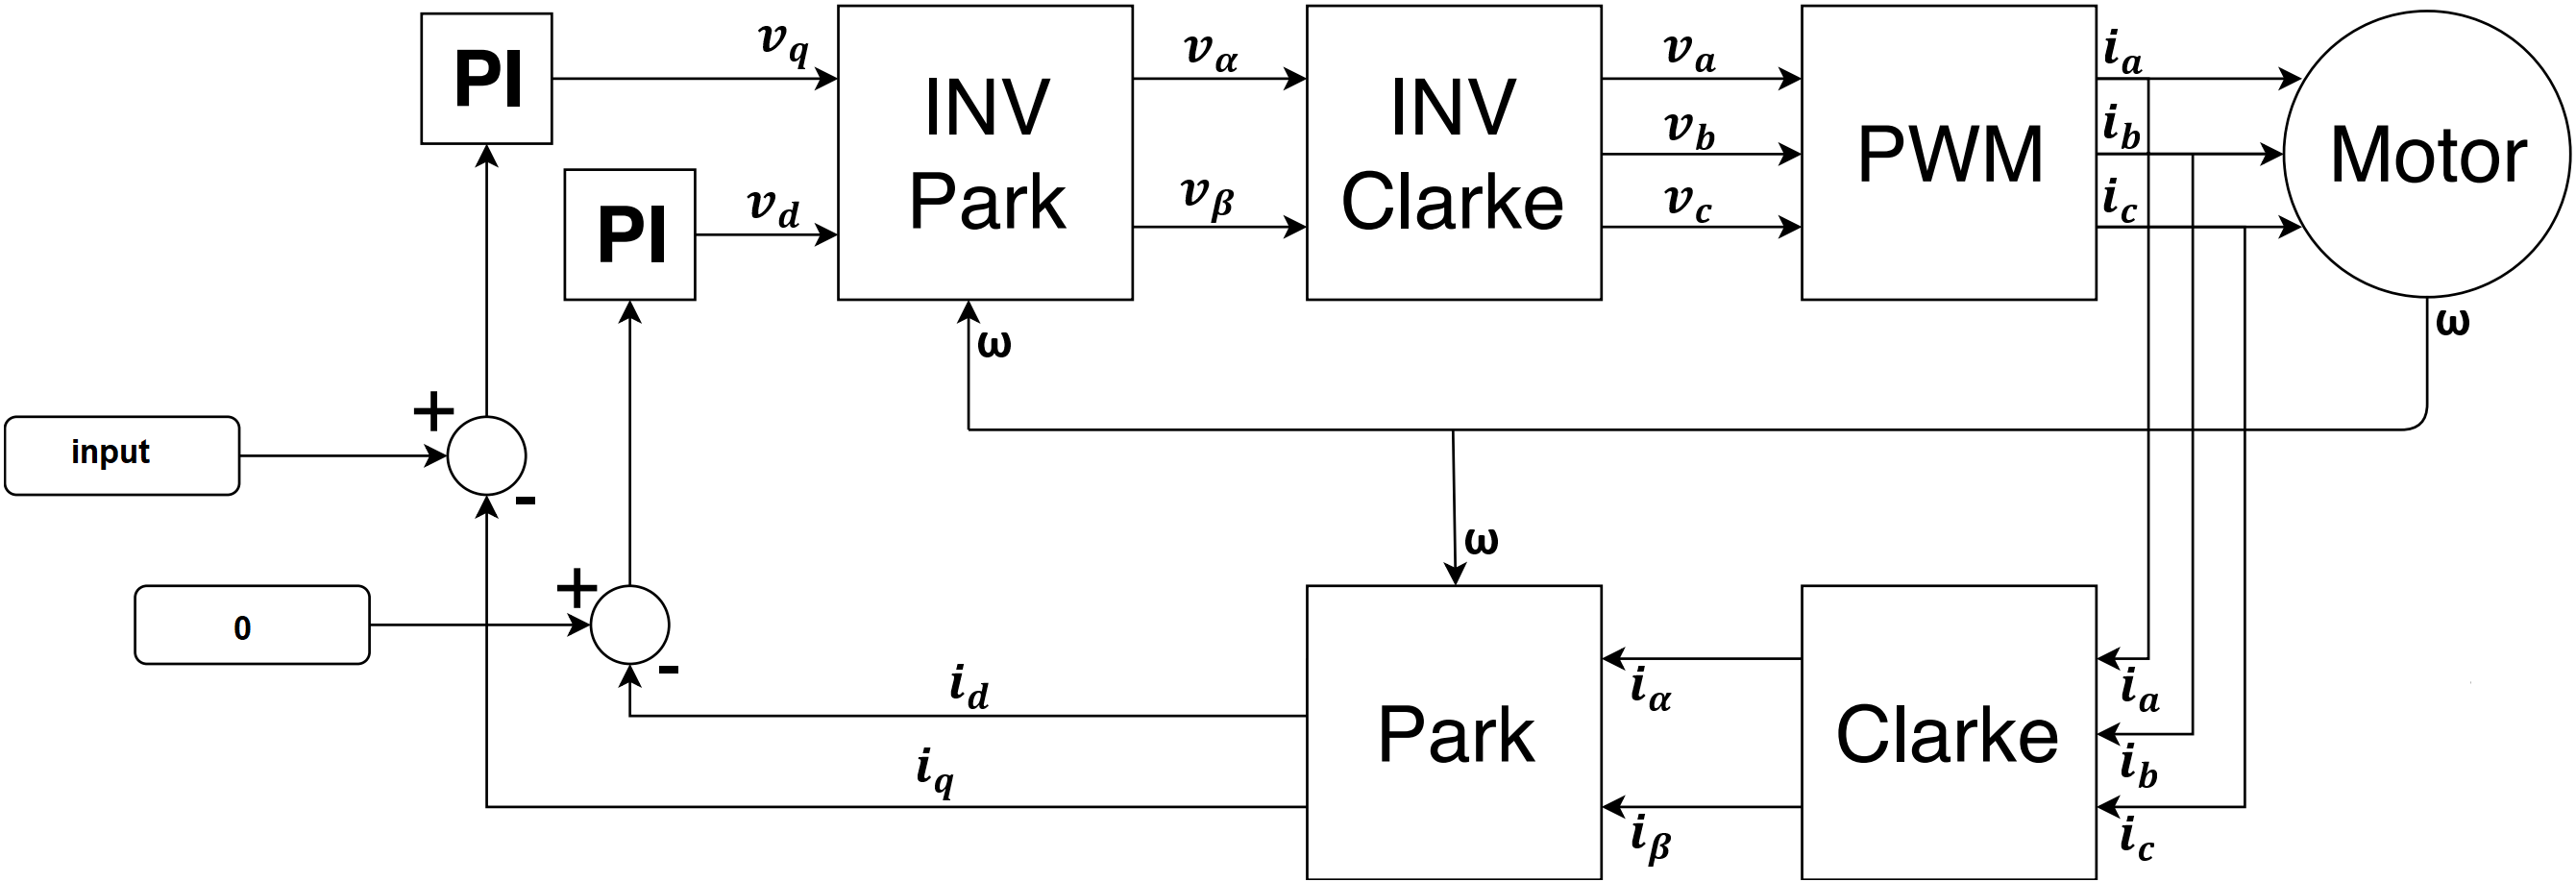
\includegraphics[scale=0.42]{pictures/control/udklip.PNG}
    \caption{Motor model used for the control as an overview.}
    \label{fig:Motor_model}
\end{figure} 

As seen in \ref{fig:Motor_model} the model consist of two inputs, two PI controllers, and inverse Park and Clarke transformations, a motor with the data from \ref{Motor_parameters_list} and negative feedback transformed back with normal Park, Clarke transformation.\\

The general idea behind model is having the input, being the wanted speed of the motor as a current, in go karts case it would be the torque pedal. The $0$ input is $0$ because of field oriented control, more on that in next section. The signal is then being tuned with the negative feedback and the controllers. Having the signal transformed is an important step, since a 3-phase motors needs 3 signals. The PWM box adjust the actual speed of the motor. The feedback comes from the 3 phases and the speed, that all help minimize errors in the signal. \\

\subsubsection{Field oriented control}
There is in motor control, a couple of common techniques used. The calculations are usually scalar based or vector based, each having their usages. In this project the technique used is FOC, which is vector based. \\

\begin{figure} [H]
    \centering
    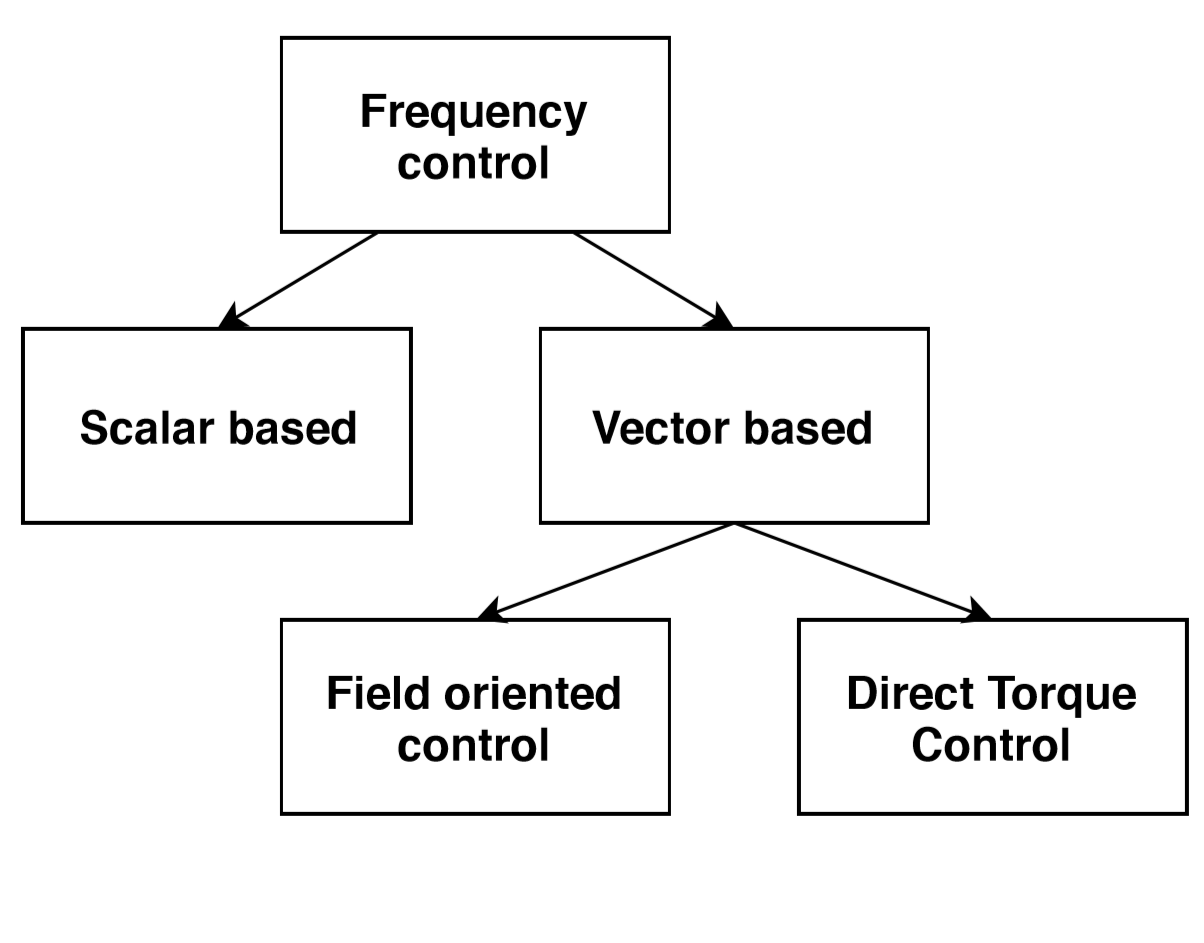
\includegraphics[scale=0.6]{pictures/control/udklip1.PNG}
    \caption{An overview of where FOC is lays among frequency control}
    \label{fig:my_label}
\end{figure} 

The reason for using FOC in this given project, is because it is relatively easy to use and implement. This method gives control over the current and voltages, and gives information about the orientation of the rotor, which gives smoother operation of the motor than normal PWM control. \\

\begin{figure} [H]
    \centering
    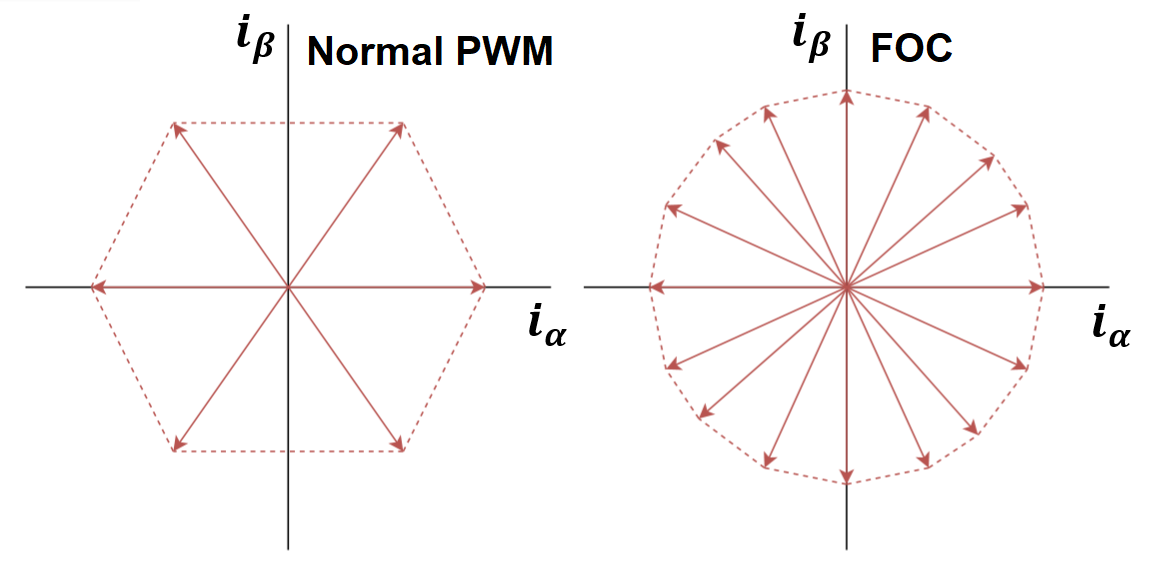
\includegraphics[scale=0.85]{pictures/control/Udklip2.PNG}
    \caption{A visualization of how FOC gives higher control of the PWM signal, the red line representing more steps of where the magnetic field can be placed.}
    \label{fig:my_label}
\end{figure}




\subsection{Clarke and Park Transformations}




% ************************** Clarke Transformation ***********************************
\subsubsection{Clarke Transformation}
The Clarke transformation converts three rotating phase currents to one rotating vector in the alpha-beta frame. The Clarke transformation is performed by using the two equations \ref{eq:clarke_transformation}.

\begin{equation}
    i_{\alpha} = \frac{2}{3} \cdot i_a - \frac{1}{3} \cdot i_b - \frac{1}{3} \cdot i_c
    , \hspace{1cm}
    i_{\beta} = 0 \cdot i_a + \frac{1}{\sqrt{3}} \cdot i_b - \frac{1}{\sqrt{3}} \cdot i_c
    \label{eq:clarke_transformation}
\end{equation}

It can also be written in matrix form as in equation \ref{eq:CtransMatrix}. 

\begin{equation}
    \centering
    \begin{bmatrix}
        i_{\alpha} \\ 
        i_{\beta}
    \end{bmatrix}
    =
    \begin{bmatrix}
        \frac{3}{2} & -\frac{1}{3} & -\frac{1}{3} \\
        0 & \frac{1}{\sqrt{3}} & -\frac{1}{\sqrt{3}} \\
    \end{bmatrix}
    \begin{bmatrix}
        i_{a} \\ 
        i_{b} \\ 
        i_{c}
    \end{bmatrix}
    \label{eq:CtransMatrix}
\end{equation}


% ************************** Park Transformation ***********************************
\subsubsection{Park Transform}
To convert the one rotating vector in the alpha-beta frame to a static vector in the rotating dp-frame, the Park transformation is used. The park transformation is performed with equtation \ref{eq:park_transformation}.

\begin{equation}
    i_{d} = cos(\varphi) \cdot i_{\alpha} + sin(\varphi) \cdot i_{\beta}
    , \hspace{1cm}
    i_{q} = -sin(\varphi) \cdot i_{\alpha} + cos(\varphi) \cdot i_{\beta}
    \label{eq:park_transformation}
\end{equation}

Where
$\omega t = \varphi$

\begin{equation}
    \centering
    \begin{bmatrix}
        i_{d} \\ 
        i_{q}
    \end{bmatrix}
    =
    \begin{bmatrix}
       cos(\omega t) & sin(\omega t) \\
       -sin(\omega t) & cos(\omega t)
    \end{bmatrix}
    \begin{bmatrix}
        i_{\alpha} \\ 
        i_{\beta}
    \end{bmatrix}
\end{equation}





% ************************** Inverse Park Transformation ***********************************
\subsubsection{Inverse Park Transform}
Converts a static vector in a rotating dq-frame into a rotating vector in a alpha-beta frame.

\begin{equation}
    \centering
    \begin{bmatrix}
        i_{\alpha} \\ 
        i_{\beta}
    \end{bmatrix}
    =
    \begin{bmatrix}
       cos(\omega t) & -sin(\omega t) \\
       sin(\omega t) & cos(\omega t)
    \end{bmatrix}
    \begin{bmatrix}
        i_{d} \\ 
        i_{q}
    \end{bmatrix}
\end{equation}

Where
$\omega t = \varphi$

\begin{equation}
    i_{\alpha} = cos(\varphi) \cdot i_{d} - sin(\varphi) \cdot i_{q}
    , \hspace{1cm}
    i_{\beta} = sin(\varphi) \cdot i_{d} + cos(\varphi) \cdot i_{q}
    \label{eq:inverse_park_transformation}
\end{equation}

% ************************** Inverse Clarke Transformation ***********************************
\subsubsection{Inverse Clarke Transform}
Converts a rotating vector in the alpha-beta frame into three phase signals. 

\begin{equation}
    \centering
    \begin{bmatrix}
        i_{a} \\ 
        i_{b} \\ 
        i_{c}
    \end{bmatrix}
    =
    \begin{bmatrix}
        1 & 0 \\
        - \frac{1}{2} & \frac{\sqrt{3}}{2} \\
        - \frac{1}{2} & - \frac{\sqrt{3}}{2}
    \end{bmatrix}
    \begin{bmatrix}
        i_{\alpha} \\ 
        i_{\beta}
    \end{bmatrix}
\end{equation}


\begin{equation}
    i_{a} = i_{\alpha}
    , \hspace{1cm}
    i_{b} = -\frac{1}{2} \cdot i_{\alpha} + \frac{\sqrt{3}}{2} \cdot i_{\beta}
    , \hspace{1cm}
    i_{c} = -\frac{1}{2} \cdot i_{\alpha} - \frac{\sqrt{3}}{2} \cdot i_{\beta}
    \label{eq:inverse_clarke_transformation}
\end{equation}

\subsection{Motor model}
A model of the motor needs to be made for the system model. The motor is a PMSM,  which means that it is driven by three phase currents. To simplify the model, the equivalent circuit for the d- and q-directions are drawn, and a model is made, based on those. In that way the PMSM can be controlled like an DC-machine.

\subsubsection{Motor model in the d-direction}
The equivalent circuit for the d-direction voltage $v_d$ of the PMSM is shown on figure \ref{fig:vd}.

\begin{figure}[H]
	\centering
	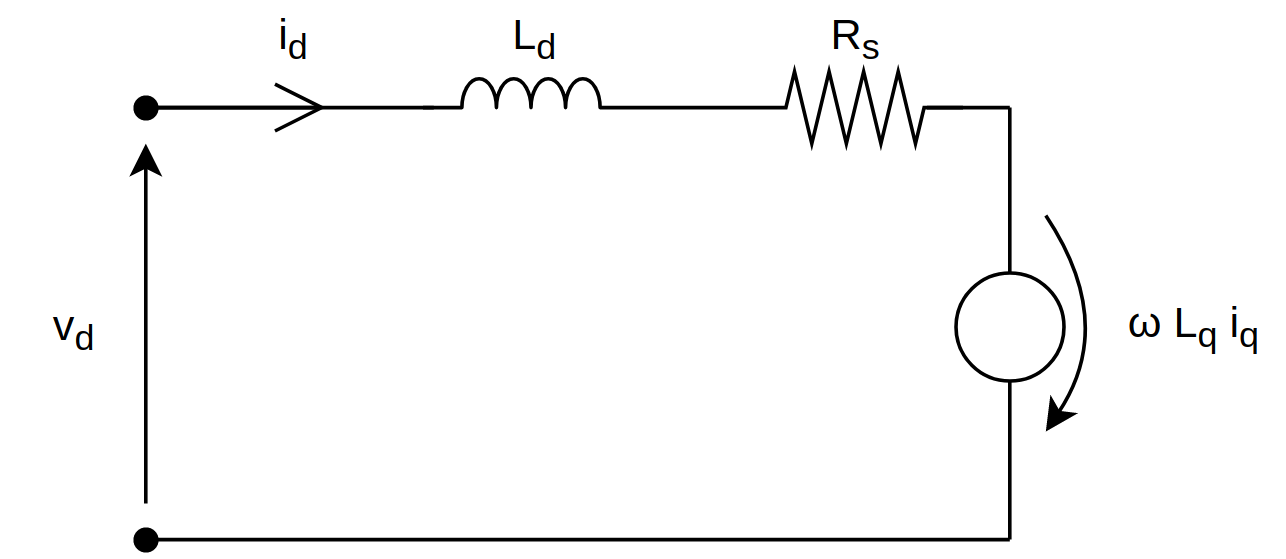
\includegraphics[width=0.6\linewidth]{pictures/control/vd}
	\caption{D-dierection equivalent circuit for the PMSM}
	\label{fig:vd}
\end{figure}


From the equivalent diagram the d-direction voltage can be described as in equation \ref{eq:d_direction}.

\begin{equation}
    \label{eq:d_direction}
    v_d = L_d \frac{d i_d}{dt} + R_s i_d - \omega L_q i_q
\end{equation}
% $\varphi_{rq} = L_qi_q$
% \begin{equation}\label{eq:d_direction2}
% v_{d} = \frac{d \varphi_{rq}}{dt} + R_s i_d - \omega \varphi_{rq}
% \end{equation}

$L_d$ and $L_q$ are respectively the d- and q-direction equivalent stator inductances for the motor, $i_d$ and $i_q$ are respectively the d- an q-direction currents, $R_s$ is the stator resistance for the motor, and $\omega$ is the rotational speed of the rotor.

If $i_d$ from the $L_d \frac{di_d}{dt}$ part is isolated and Laplace transformed it result in equation \ref{eq:d_direction}.

\begin{equation}
    \label{eq:d_direction2}
    I_d = \frac{1}{S} \frac{1}{L_d} (V_d - I_d R_d + \omega L_q I_q)
\end{equation}

From equation \ref{eq:d_direction2} the model of the d-direction of the motor is determined. That can be seen on figure \ref{fig:simulink_d_direction}.

\begin{figure}[H]
	\centering
	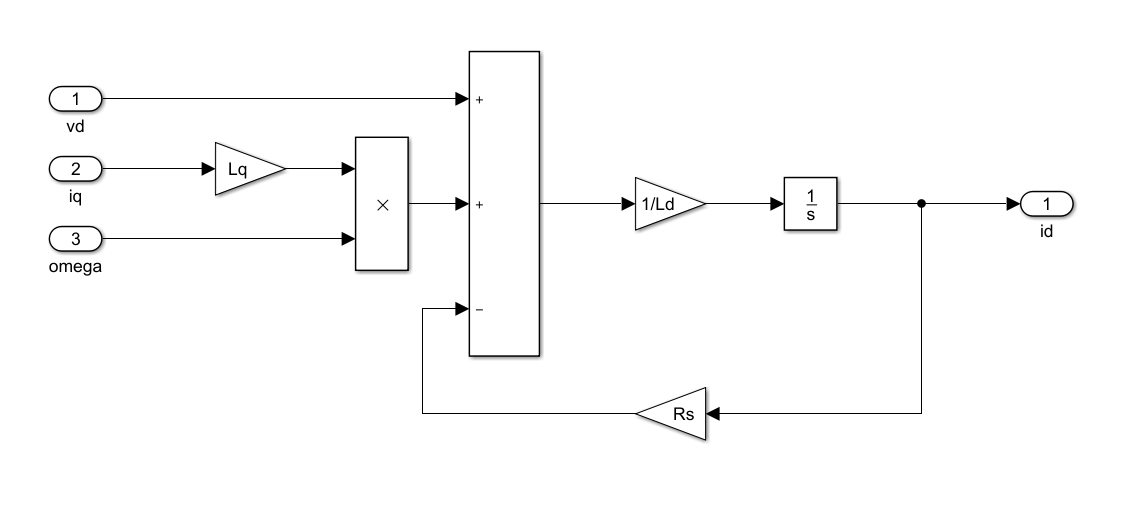
\includegraphics[width=0.8\linewidth]{pictures/control/simulink_d_direction.PNG}
	\caption{Simulink model of the d-direction of the motor model}
	\label{fig:simulink_d_direction}
\end{figure}



\subsubsection{Motor model in the q-direction}
The equivalent circuit for the q-direction voltage $v_q$ is shown on figure \ref{fig:vq}.

\begin{figure}[H]
	\centering
	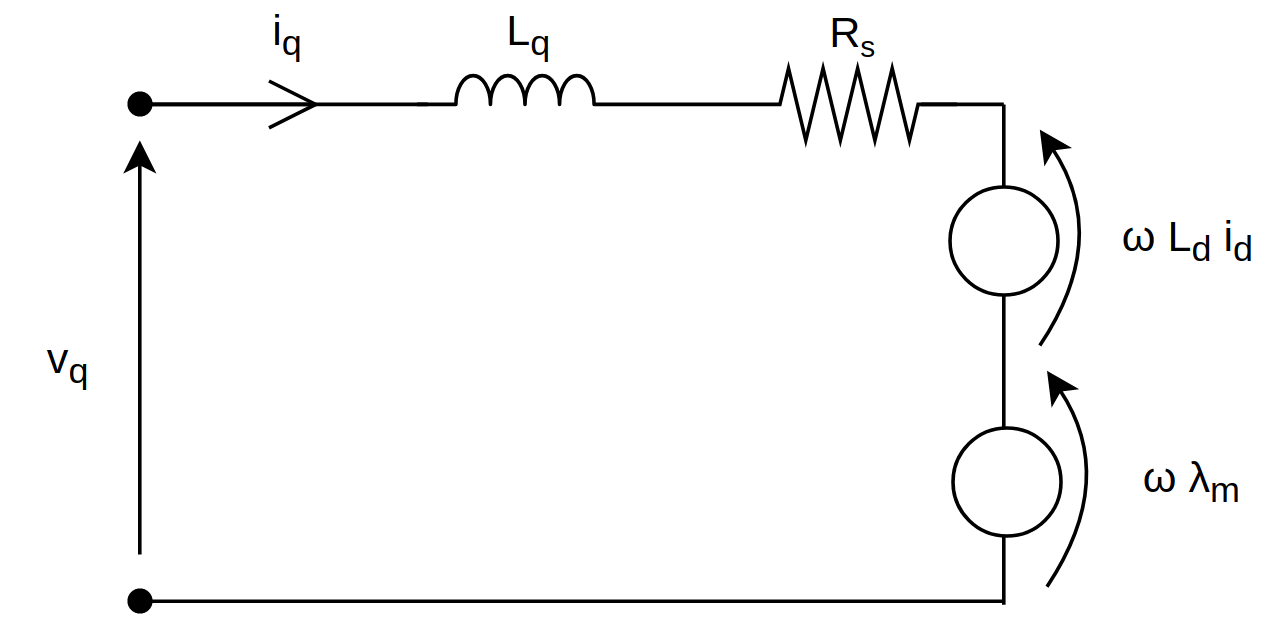
\includegraphics[width=0.6\linewidth]{pictures/control/vq.png}
	\caption{Q-direction equivalent circuit for the PMSM}
	\label{fig:vq}
\end{figure}

The voltage in the q-direction can be described from equation \ref{eq:q_direction}.

\begin{equation}
\label{eq:q_direction}
    v_q = L_q\frac{d i_q}{dt} + R_s i_q + \omega L_d i_d + \omega \lambda_m
\end{equation}

% \begin{equation}\label{eq:q_direction2}
% v_{sq} = R_si_q + \frac{d \varphi_{rd}}{dt} +  \omega_e \varphi_{rd}
% \end{equation}
% Where \\
% $\varphi_{rd} = L_di_d$

$\lambda_m$ is the flux linkage.

The $i_q$ from the $L_q \frac{di_q}{dt}$ part is isolated and Laplace transformed. This results in equation \ref{eq:d_direction}.

\begin{equation}
    \label{eq:q_direction2}
    I_q = \frac{1}{S} \frac{1}{L_q} (V_q - I_q R_q - \omega L_d I_d - \omega \lambda_m)
\end{equation}

From equation \ref{eq:q_direction2} the q-direction model can be produced. The model can be seen on figure \ref{fig:simulink_q_direction}.

\begin{figure}[H]
	\centering
	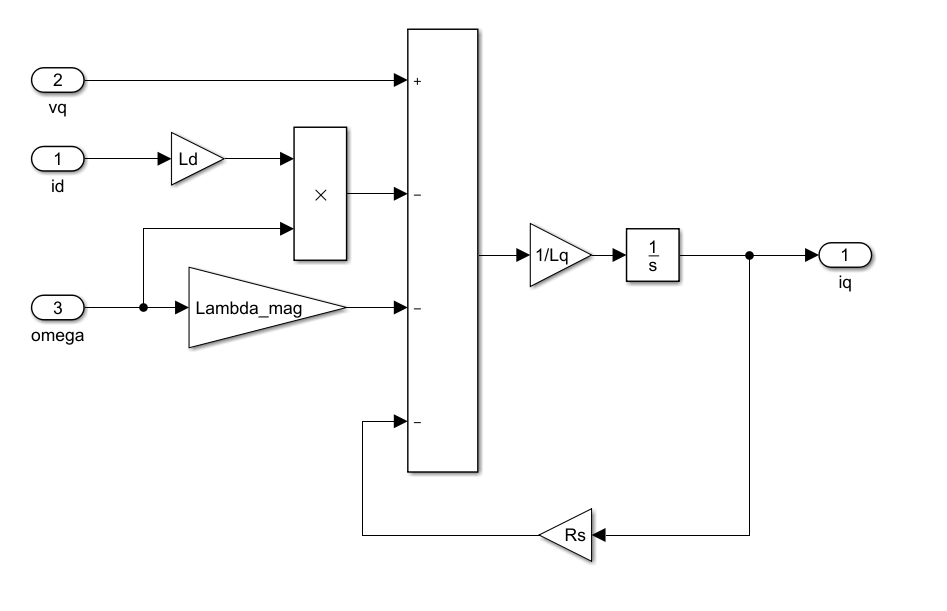
\includegraphics[width=0.8\linewidth]{pictures/control/simulink_q_direction.PNG}
	\caption{Simulink model of the q-direction of the motor model}
	\label{fig:simulink_q_direction}
\end{figure}


\subsubsection{Mechanical model}
For a multiple pole synchronous motor, the torque produced from the electrical field can be found from equation \ref{eq:torque_equation}.

\begin{equation}
    \label{eq:torque_equation}
    T_e = \frac{3P}{2} \big(\lambda_m i_{q} + (L_d - L_q) i_q i_{d}\big)
\end{equation}

Where $P$ is the number of pole pairs.

Because $L_q$ is higher than $L_d$, it can be seen from equation \ref{eq:torque_equation} the current running in the d-direction produces negative torque and is therefore reducing the output torque. 

The total torque at shaft of the motor, will be the sum of the torque the electrical field produces, the torque produces by the friction in the motor, and a possible external load torque. The total torque can be set equal to the inertia of the system multiplied with the acceleration. As seen in equation \ref{eq:total_torque}.

\begin{equation}
    \label{eq:total_torque}
    J\frac{d\omega}{dt} = T_e - B\omega - T_{load}
\end{equation}

$J$ is the inertia, $B$ is the friction coefficient, and $T_{load}$ is the torque from the external load.
Equation \ref{eq:total_torque} is rewritten and combined with equation \ref{eq:torque_equation} to a equation for the rotational speed. This is Laplace transformed, and the result is equation \ref{eq:omega}.

\begin{equation}
    \label{eq:omega}
    \omega = \frac{1}{S} \frac{1}{J} \bigg( \frac{3P}{2} \big( \lambda_m I_q + (L_d - L_q) I_q I_d \big) - B\omega - T_{load} \bigg)
\end{equation}

From equation \ref{eq:omega} can a model with the torque, rotational speed, and the angle of the motor as output, and the d- and q-current as inputs. This model can be seen on figure \ref{fig:torque}.

\begin{figure}[H]
	\centering
	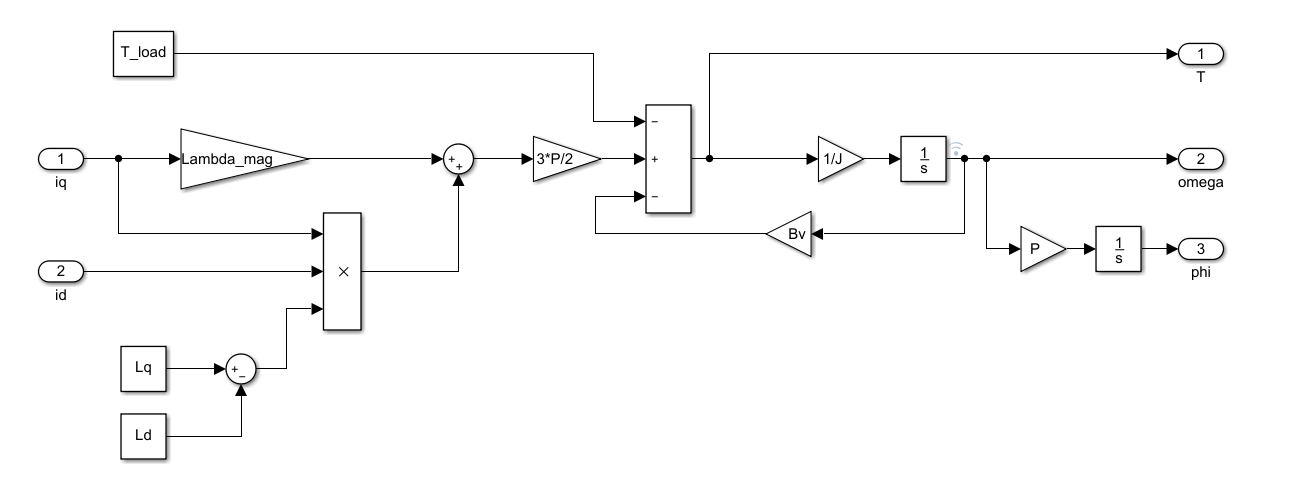
\includegraphics[width=1\linewidth]{pictures/control/torque.PNG}
	\caption{Simulink model of the motor with torque, rotational speed and the position of the rotor as output and the the d- and q-current as input}
	\label{fig:torque}
\end{figure}

\subsubsection{Complete motor model}
The three models, for the d-direction, the q-direction and the mechanical part, are put into subsystems and connected. This can be seen on figure \ref{fig:motor}

\begin{figure}[H]
	\centering
	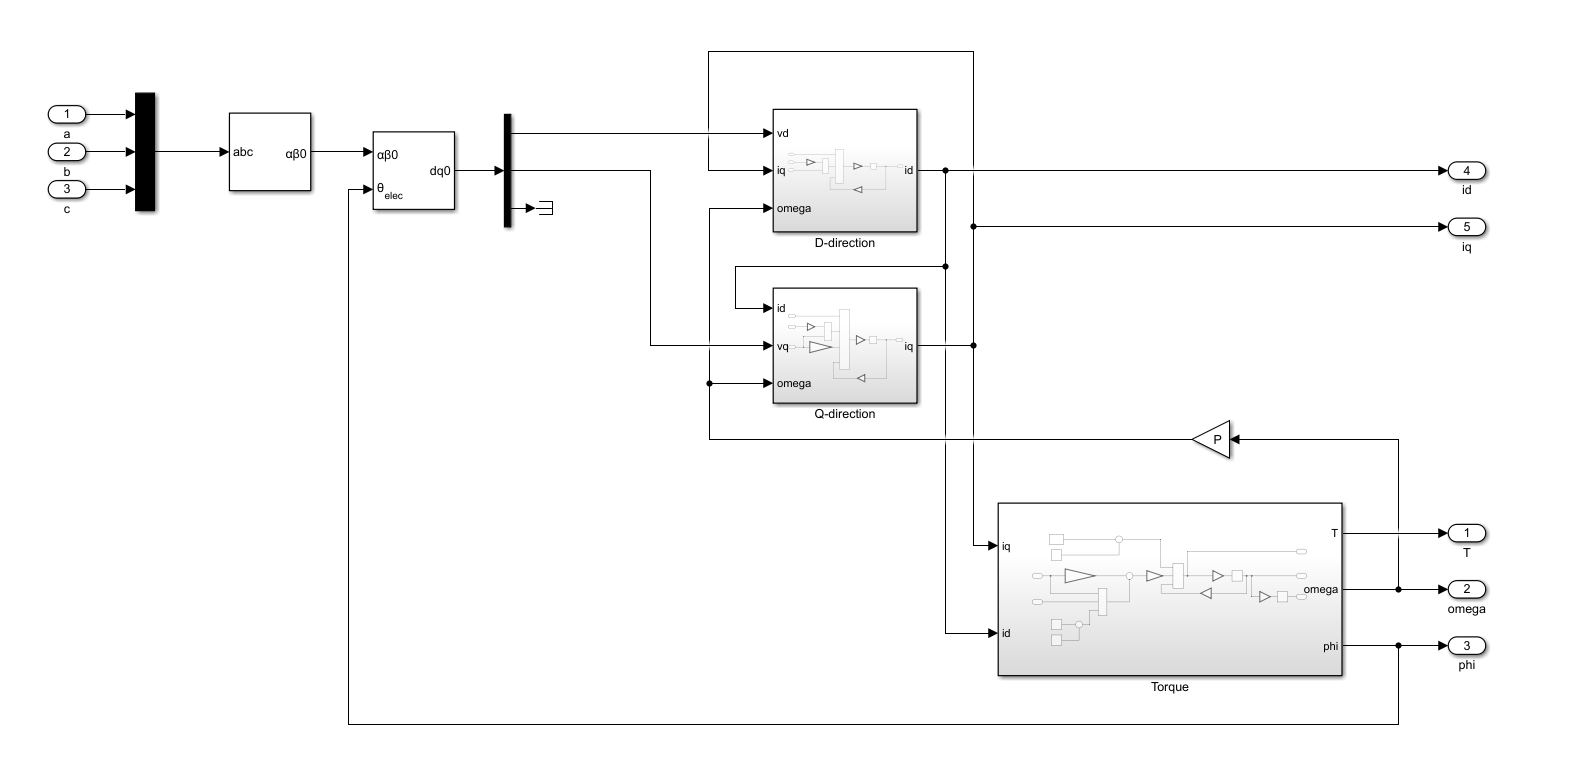
\includegraphics[width=1\linewidth]{pictures/control/motor_model.PNG}
	\caption{Simulink model of the full motor model}
	\label{fig:motor}
\end{figure}

Because the motor model is in the dq-frame, the three rotational phases voltages is converted to the dq-frame in the beginning of the model. The model outputs the d- and q-current, the torque, speed and angle of the motor. The rotational speed outputted from the motor model is the mechanical speed, and is therefore converted to the electrical speed before it is inputted to the d- and q-models. 



\subsection{Control system}
\label{sec:control_system}

For controlling the motor, the output d- and q-current of the motor are feedback to a PI-controller for each of them. The d-current is desired to be zero, and is therefore compared with zero before the PI-controller. The q-current is desired to be set to the reference point set by the input from the torque pedal. The torque reference input is therefore converted to a current, which can be compared with the feedback q-current from the motor model.

After the PI-controller the d- and q-voltages are converted back into three phases with an Inverse Clarke and an Inverse Park transformation. The three phase voltages are then put into the motor model.

The full model of the system can be seen on figure \ref{fig:control_system}.


\begin{figure}[H]
	\centering
	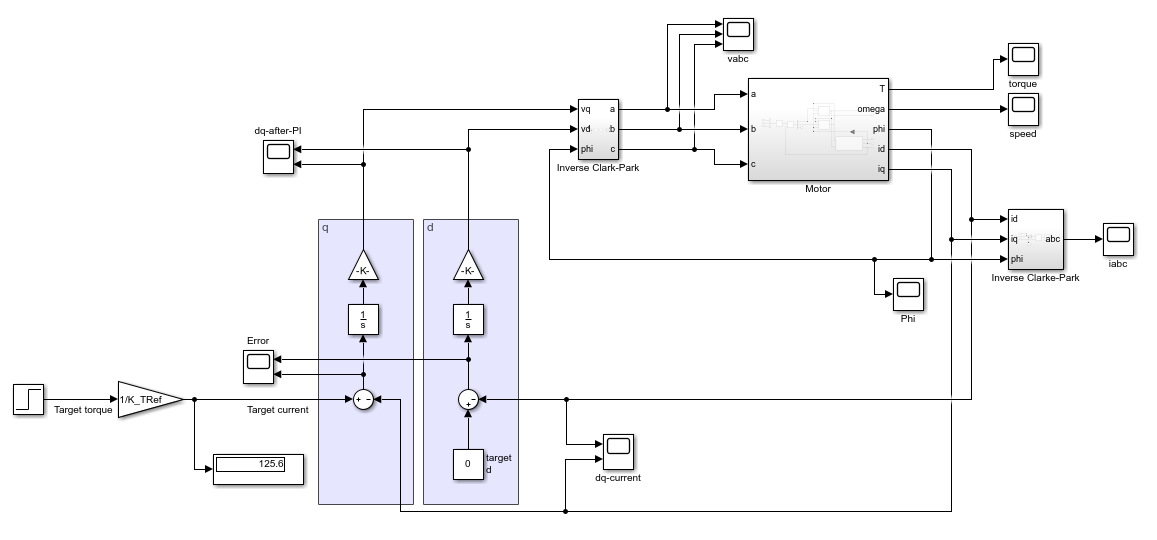
\includegraphics[width=1\linewidth]{pictures/control/full_model.PNG}
	\caption{The entire control model, with PI controller and motor model.}
	\label{fig:control_system}
\end{figure}



\subsection{PI-controller}

To set the PI-controller the transfer functions for the d- and q-direction is determined, with the voltages as input and the current as output. This is done based on the equations for the voltages in the d- and q-direction, equation \ref{eq:d_direction} and \ref{eq:q_direction}.
Because a transfer function only can have one input and one output, the two equation, \ref{eq:d_direction} and \ref{eq:q_direction}, is shortened. The new equation can be seen in equation \ref{eq:d_direction3} and \ref{eq:q_direction3}.

\begin{equation}
    \label{eq:d_direction3}
    v_d = L_d \frac{d i_d}{dt} + R_s i_d
\end{equation}

\begin{equation}
    \label{eq:q_direction3}
    v_q = L_q \frac{d i_q}{dt} + R_s i_q
\end{equation}

As seen in the two equations, \ref{eq:d_direction3} and \ref{eq:q_direction3}, the parts in the equations depending on other variables than the current is neglected. 
This Laplace transformed and converted to the transfer functions for the two systems.

\begin{equation}
    \frac{I_d(s)}{V_d(s)} = \frac{ \frac{1}{ \frac{L_d}{R_s} } }{ \frac{R_s}{ \frac{L_d}{R_s} } + R_s s }
\end{equation}

\subsection{Simulation}
\label{sec:simulation}
The model is tested with a step from $0$ to $47.8 Nm$, which correspond to a target q-current of $300 A $. At the start the load torque is set to $20 Nm$, and after $0.5 s$ it is increased to $40 Nm$. 

The three phase currents produced can be seen on figure \ref{fig:iabc}.

\begin{figure}[H]
	\centering
	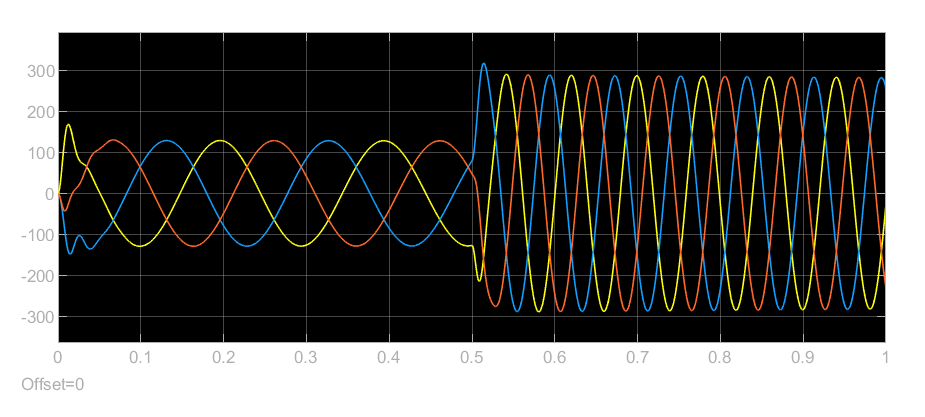
\includegraphics[width=0.6\linewidth]{pictures/control/iabc.eps}
	\caption{The ABC current from the motor model}
	\label{fig:iabc}
\end{figure}

As it it seen in figure \ref{fig:iabc}, the amplitude of the current increases when a bigger load is put on the motor. 
% A higher demand of current was expected when a bigger load is put on the motor. 

The d- and q-current can be seen on figure \ref{fig:idq}.

\begin{figure}[H]
	\centering
	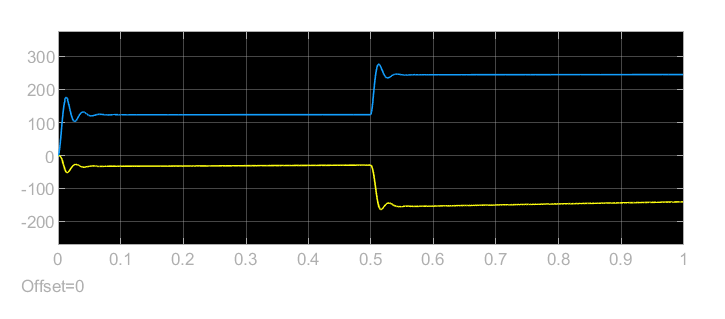
\includegraphics[width=0.6\linewidth]{pictures/control/idq.eps}
	\caption{The d- and q-current from the motor model. The yellow curve is the d-current and the blue curve is the q-current}
	\label{fig:idq}
\end{figure}

On figure \ref{fig:idq} it can be seen that the q-current is not going toward the set reference. It can also be seen that the d-current is very slowly going towards zero.

On the figure \ref{fig:speed} and \ref{fig:torque} the speed and the torque of the motor can be seen.

\begin{figure}[H]
	\centering
	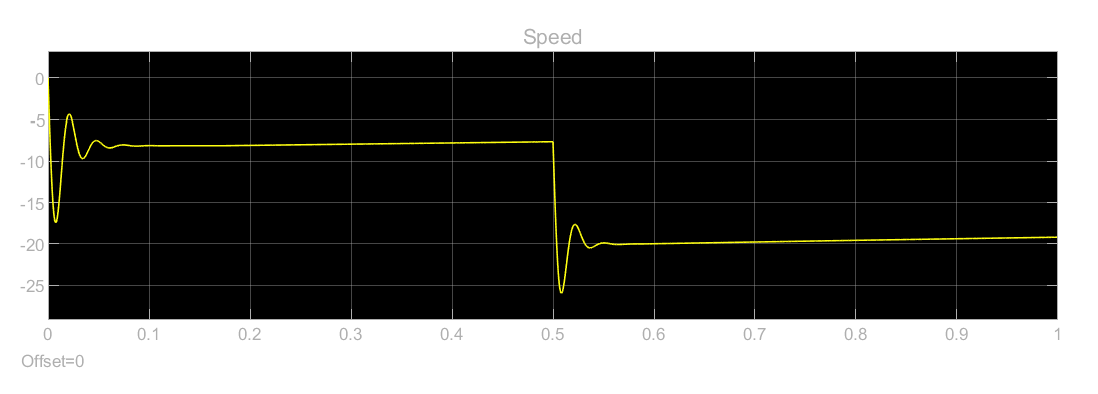
\includegraphics[width=0.7\linewidth]{pictures/control/speed.eps}
	\caption{The speed of the motor}
	\label{fig:speed}
\end{figure}

\begin{figure}[H]
	\centering
	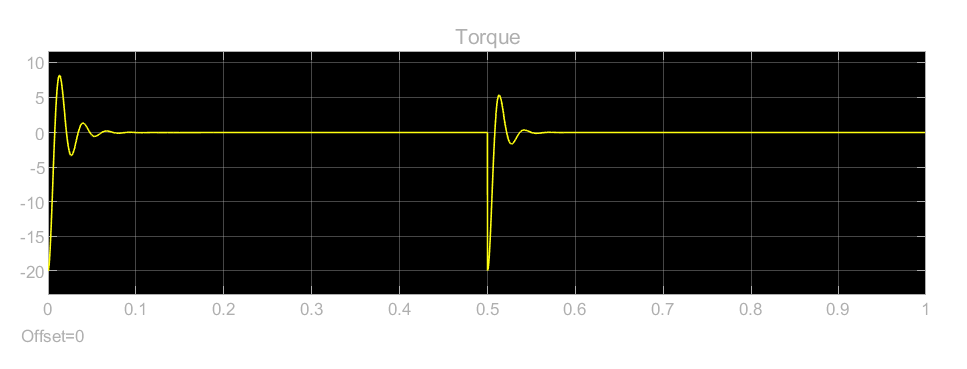
\includegraphics[width=0.7\linewidth]{pictures/control/torque.eps}
	\caption{The torque of the motor}
	\label{fig:torque}
\end{figure}



\subsection*{Subconclusion}
A model of the PMSM is made in the dq-frame, and it is controlled with field orientated control. For converting the three rotating phases going into the motor, to a d- and q-vector in a rotating frame, the Clarke and Park transformation is used. A PI-controller is used to control the d- and q-currents in the motor. Some minor problems have resulted in the model not working as expected. 

